\documentclass[generalized_symmetry.tex]{subfiles}
\setcounter{chapter}{4}
\begin{document}

\chapter{高次元の非可逆対称性}
高次元の非可逆対称性は比較的新しい話題で、現在も盛んに研究が進んでいる分野です。高次元の非可逆対称性の系統的な調べ方はまだありません。いくつかの例が知られているだけです。高次元の非可逆対称性の発見の仕方にはいくつかあります。例えば次のような方法があります。
\begin{itemize}
  \item 高次ゲージ化(higher gauging)
  \item 半空間ゲージ化(half-space gauging)
\end{itemize}
後者は\ref{sec:KWdefect}節でKramers-Wannier双対性の欠陥を作るのに用いた方法の高次元版です。この講義では、この後この半空間ゲージ化について詳しく紹介します。名前を見て分かるとおり、両方とも「ゲージ化」の方法ですので、まずは高次形式対称性のゲージ化について説明します。

\section{高次形式対称性のゲージ化}
$G$を有限アーベル群とし、$\Tcal$を$d$次元の場の理論で$p$形式$G$対称性($G^{(p)}$対称性)を持つものとします。$X$を$d$次元の向きのついた閉リーマン多様体とします。$K$を$X$の単体分割とします。
この単体分割を利用して$G^{(p)}$対称性に対する背景ゲージ場を$A\in Z^{p+1}(X;G)$として導入します。この背景ゲージ場のもとでの分配関数を$Z_{\Tcal}(A)$と表します。

\subsection{ゲージ化した理論の分配関数}

$Z_{\Tcal}(A)$がアノマリーが無い場合、つまり$Z_{\Tcal}(A+\delta \lambda)=Z_{\Tcal}(A)$が成り立ち、しかも単体分割のしかた$K$に依存しない場合を考えます。このとき、ゲージ化した理論$\Tcal/G^{(p)}$を考えることができます。その分配関数$Z_{\Tcal/G^{(p)}}(A)$はすべてのゲージ場の配位について足し合わせることで得られます。
\begin{align}
  Z_{\Tcal/G^{(p)}} = \frac{1}{\mathrm{Vol}} \sum_{a \in Z^{p+1}(X;G)} Z_{\Tcal}(a).
  \label{gaugingincochain}
\end{align}
ここで$\mathrm{Vol}$はゲージ体積であり、ゲージ変換でつながるようなゲージ場の配位を何回も数えている分を割っておくものです。

ゲージ体積について少し考えてみます。以下、式を短くするために$C^p(K,G)$のことを引数を省略して単に$C^p$と書くことにします。素朴にはゲージ変換のパラメーター$\lambda \in C^{p}$の数なので$1/\mathrm{Vol} = 1/|C^p|$と考えられます。しかし、$\lambda \in C^p$がすべて独立なゲージ変換のパラメーターではなく、$\lambda\in C^p$と$\lambda+d\sigma$, $\sigma \in C^{p-1}$は同じゲージ変換を表しますので、$|C^{p-1}|$で割る必要があります。しかし、話はこれで終わりではなく、$\sigma \in C^{p-1}$もすべて独立なパラメーターではなく……と続けていく必要があります。最終的には
\begin{align}
  \frac{1}{\mathrm{Vol}} =
  \begin{cases}
    \frac{|C^{p-1}||C^{p-3}|\dots 1}{|C^p||C^{p-2}|\dots |C^0|}  & (p \text{ が偶数のとき}) \\
    \frac{|C^{p-1}||C^{p-3}|\dots |C^0|}{|C^p||C^{p-2}|\dots 1}  & (p \text{ が奇数のとき})  
  \end{cases}
  \label{gaugevolcochain}
\end{align}
となります。

文献等ではこれらはコチェイン$C^*$の言葉ではなくてコホモロジーの言葉で書いてあることも多いと思います。それについてここで説明します。まず、$H^{p+1}=Z^{p+1}/B^{p+1}$なので、
\begin{align}
  \sum_{a \in Z^{p+1}(X;G)} Z_{\Tcal}(a)=|B^{p+1}|\sum_{a \in H^{p+1}} Z_{\Tcal}(a)\label{gaugingtemp}
\end{align}
となります。また、完全系列(前の写像の像が次の写像の核になるような系列)
\begin{align}
  0 \to Z^{p} \overset{i}{\to} C^{p} \overset{\delta}{\to} B^{p+1} \overset{\delta}{\to} 0 
\end{align}
を考えることができます。ここで$i$は包含写像です。この完全系列から
\begin{align}
  B^{p+1}=C^{p}/Z^{p}
\end{align}
であることが分かります。これらの関係を用いると
\begin{align}
  |B^{p+1}|&=\frac{|C^{p}|}{|Z^{p}|}
  =\frac{|C^{p}|}{|H^p||B^p|}=\frac{|C^{p}||Z^{p-1}|}{|H^p||C^{p-1}|}
  =\frac{|C^{p}||H^{p-1}||B^{p-1}|}{|H^p||C^{p-1}|}
  =\dots\\
  &=\frac{|C^{p}||C^{p-2}|\dots }{|C^{p-1}||C^{p-3}|\dots}\times
  \frac{|H^{p-1}||H^{p-3}|\dots }{|H^p||H^{p-2}|\dots } 
\end{align}
となります。これを\eqref{gaugingtemp}に代入し、さらに\eqref{gaugingincochain}、\eqref{gaugevolcochain}を用いると
\begin{align}
  Z_{\Tcal/G^{(p)}} = \frac{|H^{p-1}||H^{p-3}|\dots }{|H^p||H^{p-2}|\dots } \sum_{a \in H^{p+1}} Z_{\Tcal}(a)
\end{align}
という表式を得ます。この他に重力に関する局所項を入れることもできます。

\subsection{双対対称性}
2次元の場合と同様に有限アーベル群$G$の$p$形式対称性をゲージ化した理論$\Tcal/G^{(p)}$には双対対称性が存在します。これについて見ていくことにしましょう。

双対対称性のトポロジカル欠陥はWilsonサーフェスと呼ばれる演算子です。これは$\rho\in \hat{G}$(1次元ユニタリー表現)つまり$\rho:G\to \U(1)$(準同型)、$c \in Z_{p+1}(K,\Zb)$として
\begin{align}
  W_{\rho}(c) = \rho\left(\int_{c} a\right)
\end{align}
を挿入することです。この欠陥は$p+1$次元ですから、余次元は$d-p-1$次元になります。つまりこれは$(d-p-2)$形式対称性のトポロジカル欠陥になります。まとめると、次のことが言えました。
\begin{emphasize}
  $\Tcal/G^{(p)}$は$\hat{G}^{(d-p-2)}$対称性を持つ。
\end{emphasize}

これをさらに詳しく見るために$G=\Zb_N$の場合に限って考えます。この場合、$q=d-p-2$としてWilsonループの情報は$B \in H^{q+1}$で表されます。この背景での分配関数は
\begin{align}
  Z_{\Tcal/G^{(p)}}(B) = \frac{|H^{p-1}||H^{p-3}|\dots }{|H^p||H^{p-2}|\dots } \sum_{a \in H^{p+1}} Z_{\Tcal}(a) \exp\left(\frac{2\pi i}{N}\int_{X} B\cupp a\right)
\end{align}
となります。ゲージ化すると、分配関数はだいたいFourier変換したようなものになります。

この$\hat{G}^{q}$対称性をゲージ化した理論$\Tcal/G^{p}/\hat{G}^q$を考えます。この分配関数は
\begin{align}
  Z_{\Tcal/G^{(p)}/\hat{G}^{(q)}} =& \frac{|H^{q-1}||H^{q-3}|\dots }{|H^q||H^{q-2}|\dots } \sum_{c \in H^{p+1}} Z_{\Tcal/\hat{G}^{q}}(b)\notag\\
  =&\frac{|H^{q-1}||H^{q-3}|\dots }{|H^q||H^{q-2}|\dots } \sum_{b \in H^{q+1}} \frac{|H^{p-1}||H^{p-3}|\dots }{|H^p||H^{p-2}|\dots } \sum_{a \in H^{p+1}} Z_{\Tcal}(a) \exp\left(\frac{2\pi i}{N}\int_{X} b\cupp a\right)
\end{align}
となります。ここで、知られている恒等式
\begin{align}
  \sum_{b \in H^{q+1}}\exp\left(\frac{2\pi i}{N}\int_{X} b\cupp a\right)=
  |H^{p+1}|\delta_{a,0}
  \label{completenessidentity}
\end{align}
を用いると
\begin{align}
  Z_{\Tcal/G^{(p)}/\hat{G}^{(q)}} =& \Ccal Z_{\Tcal},\\
  \Ccal=&
  \frac{|H^{q+1}||H^{q-1}||H^{q-3}|\dots }{|H^q||H^{q-2}|\dots }\frac{|H^{p-1}||H^{p-3}|\dots }{|H^p||H^{p-2}|\dots } 
\end{align}
を得ます。つまり$\Tcal/G^{(p)}/\hat{G}^{(q)}$の分配関数と$\Tcal$の分配関数は比例係数を除いて等しいので、これら2つの理論は同じであることが期待できます。

これらをもう少し精密にするために、比例係数についてもう少し詳しく見ていきます。これも一般にやるのは少し大変なので、$X$にトーションが無い場合、つまり$H^{*}(X,\Zb)$の$0$でない元を$0$でないどんな整数倍しても$0$でないような場合を考えます。このときある非負の整数$b_p$があって$H^{p}(X,\Zb)\cong \Zb^{b_p}$となります。この$b_p$を用いて$H^{p}(X,G)\cong G^{b_p}$と書けるので$|H^{p}|=N^{b_p}$となります。また、$b_{d-p}=b_p$であることも知られています。
$p=d-q-2$であることも思い出すと比例係数は
\begin{align}
  \Ccal=
  \begin{cases}
    N^{\chi}& (q \text{ が偶数のとき}) \\
    N^{-\chi}& (q \text{ が奇数のとき})
  \end{cases}
\end{align}
となります。ここで
\begin{align}
  \chi = \sum_{p=0}^{d}(-1)^p b_p
\end{align}
はEuler数です。$d$が奇数のときは$\chi=0$になりますので、$\Ccal=1$となります。$d$が偶数のときには、ゲージ化した分配関数を先ほどの定義から
\begin{align}
  Z^{\text{new}}_{\Tcal/G^{(p)}} = \sqrt{\Ccal} Z^{\text{old}}_{\Tcal/G^{(p)}}
  \label{Eulercountertermgeneral}
\end{align}
とすることにより$Z_{\Tcal/G^{(p)}/\hat{G}^{(q)}} = Z_{\Tcal}$となるようにすることができます。\eqref{Eulercountertermgeneral}の再定義は作用に局所的な項を付け加えることで実現できます。これはEulerの公式
\begin{align}
  \chi=\sum_{r=0}^{d}(-1)^r (\text{$r$単体の数})
\end{align}
を用いると分かります。実際、各$r$単体に対して
\begin{align}
  \begin{cases}
    \sqrt{N}^{(-1)^r} & (\text{$p$,$q$が偶数のとき}) \\
    \sqrt{N}^{(-1)^{r+1}} & (\text{$p$,$q$が奇数のとき})
  \end{cases}
\end{align}
の因子をかければ良いことになります。

さらに、背景ゲージ場を入れた場合にも同様の解析ができます。このとき、
\begin{align}
  Z_{\Tcal/G^{(p)}/\hat{G}^{(q)}}(A)=(\text{定数})\sum_{b\in H^{q+1}}\sum_{a \in H^{p+1}} Z_{\Tcal}(a) \exp\left(\frac{2\pi i}{N}\int_{X} A\cupp b\right)\exp\left(\frac{2\pi i}{N}\int_{X} b\cupp a\right)
\end{align}
となります。ここで
\begin{align}
  b\cupp a = (-1)^{(p+1)(q+1)} a \cupp b
\end{align}
であることを思い出して、\eqref{completenessidentity}を用いると
\begin{align}
  Z_{\Tcal/G^{(p)}/\hat{G}^{(q)}} (a) =
  \begin{cases}
    Z_{\Tcal}(-a) & ( \text{$p$, $q$ がともに偶数のとき}) \\
    Z_{\Tcal}(a) & (\text{それ以外})
  \end{cases} 
\end{align}
を得ます。$p$,$q$がともに偶数のときの背景ゲージ場の符号が反転していますが、これは荷電共役をとった理論になります。したがって、次のことが言えました。
\begin{emphasize}
  $\Tcal/G^{(p)}/\hat{G}^{(q)}$は、$\Tcal$あるいはその荷電共役と同じ理論である。  
\end{emphasize}

さて2回ゲージ化して同じ理論に戻るなら、特殊な場合には1回ゲージ化しても同じ理論に戻るということがありえます。この場合には$p=q$である必要があります。つまり$d=2n$としたとき$p=q=n-1$の場合です。$n=1$の場合の例は前に詳しくやったKW双対性です。次に簡単なのは$n=2$の場合です。つまり4次元で$\Tcal/G^{(1)}\cong\Tcal$になる場合がありえます。例を挙げると
\begin{itemize}
  \item $\Ztwo$格子ゲージ理論、$K=K_c$の場合のKramarse-Wannier-Wegner(KWW)双対性。
  \item Maxwell理論で$\frac{1}{g^2}=\frac{N}{4\pi}$のときの電磁双対性。
  \item $\Ncal=4$超対称Yang-Millsでゲージ群が$\SU(N)$、coupling が$\tau=i$の場合のMontonen-Olive双対性。
\end{itemize}
このような場合には2次元のときと同様にして半空間ゲージ化によってトポロジカル欠陥を作ることができます。一般にはこれは非可逆対称性になります。このようにして作られるトポロジカル欠陥は双対性欠陥と呼ばれます。この講義の残りで、上2つの例:$\Ztwo$格子ゲージ理論とMaxwell理論の双対性欠陥について説明します。

\section{4次元\texorpdfstring{\Ztwo}{Z2}格子ゲージ理論}

1つ目の例は我々が\cite{Koide:2021zxj}でやったものです。これは2次元のKW双対性の4次元のアナロジーです。第\ref{ch:Ising}章でやったのと同様の解析によりその性質を調べることができます。ここではその内容を簡単に説明します。

考える理論は4次元$\Ztwo$格子ゲージ理論で、これは\ref{subsec:latticegauge}項で取り扱った格子ゲージ理論においてゲージ群を$\SU(N)$の代わりに$\Ztwo$としたものです。つまり4次元の立方格子において、各リンク$\ell$に$\Ztwo$の元$a_{\ell}=0,1$を割り当てます。分配関数は$K$を正の実数の定数として
\begin{align}
  Z_{\Tcal}(K)=\sum_{\{a\}} \exp\left(K\sum_{\text{すべてのプラケット}\expval{1234}}(-1)^{a_1+a_2+a_3+a_4}\right)
\end{align}
と書けます。Ising模型と似ているのが分かってもらえるでしょうか。

この理論には中心対称性$\Ztwo^{(1)}$があります。これは\ref{sec:latticecentersymmetry}節で説明したとおりのものです。中心対称性$\Ztwo^{(1)}$は2次元Ising模型のときのスピン反転対称性のアナロジーです。

さらに、この理論にはKW双対性に似た双対性であるKWW双対性があります。これの主張は適切な局所相殺項を加えると
\begin{align}
  Z_{\Tcal/\Zb_{2}^{(1)}}(K) = Z_{\Tcal}(\Kt),\quad \sinh 2K \sinh 2\Kt=1
\end{align}
となることです。この関係は2次元のIsing模型のKW双対性と同様の方法で示すことができます。特に$K=\Kt$のとき、つまり$K=K_c:=\frac{1}{2}\log(1+\sqrt{2})$のときには、$\Tcal$と$\Tcal/\Zb_{2}^{(1)}$は同じ理論になります。これは2次元Ising模型の臨界点と同じです。

この理論の相構造について見ておきます。用語など、適宜\ref{sec:phasestructure}を参照してください。まず、極端な場合について考えておきます。
\begin{itemize}
  \item $K\ll 1$(強結合)のとき、強結合展開により、Wilsonループは面積則であることが分かります。つまり、閉じ込め相であり、$\Ztwo^{(1)}$対称性が保たれている相です。真空は唯一であり、自明にギャップがある相です。
  \item $K\gg 1$(弱結合)のとき、flatな配位が支配的になり、Wilsonループは自明に$1$になります。つまり、非閉じ込め相であり、$\Ztwo^{(1)}$対称性が自発的に破れている相です。ギャップはあいていますが、空間のトポロジーによって真空に有限個の縮退があるトポロジカル秩序相になります。
\end{itemize}
これらは対称性が異なる相なので相転移は必ずあります。2次元Isingと同様の双対性を用いた論理で、相転移が一回だけあるとすると、それは自己双対の点$K=K_c$であることが分かります。これらをまとめると図\ref{fig:z2latticephasestructure}のようになります。これも2次元Ising模型の相構造と似ています。

\begin{figure}[htbp]
  \centering
  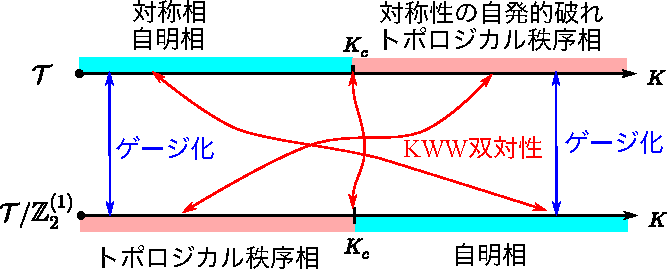
\includegraphics{z2latticephasestructure.pdf}
  \caption{$\Ztwo$格子ゲージ理論の相構造の図。}
  \label{fig:z2latticephasestructure}
\end{figure}

2次元Isingの場合と異なるところは、相転移の次数です。2次元Ising模型の相転移は二次相転移でしたが、$\Ztwo$格子ゲージ理論の相転移は一次相転移です。これは昔Creutzが数値計算により発見したものです。相転移が一次ですから、相転移点直上でもギャップがある理論になっているので、この相転移点を利用してトポロジカルでない連続理論を作ることはできません。

$K=K_c$のときには、$\Tcal$と$\Tcal/\Zb_{2}^{(1)}$は同じ理論になります。このとき、2次元の場合と同様にして半空間ゲージ化によりトポロジカル欠陥「双対性欠陥」を作ることができます。こうしてできる双対性欠陥は余次元1で、中心対称性の欠陥$\Zb_{2}^{(1)}$と合わせて様々な演算ができます。特に双対性欠陥の量子次元に当たる量($S^3$の分配関数)は$1/\sqrt{2}$になります。このことから双対性欠陥が非可逆であることが分かります。

\section{Maxwell理論}

別の双対性欠陥の例として、4次元Maxwell理論の電磁双対性から来る双対性欠陥を考えます。Maxwell理論には電場と磁場を入れ替える双対性がありますが、まずそれを精密に定式化します。その後で双対性欠陥を作る方法を説明します。

\subsection{Maxwell理論}
まず、Maxwell理論の作用を書きます。$X$を閉Riemann多様体(正定値計量$g_{\mu\nu}$の入った多様体)でスピン構造が入っているとします\footnote{ボゾンだけの理論なのに、なぜスピン構造が必要なのかは、かなり技術的です。スピン構造が無い場合にも双対性を議論できますが、その場合の双対性の構造はかなりややこしいものになるので、この講義では取り扱いません。}。ベクトルポテンシャルを$A=A_{\mu}dx^{\mu}$とし、$F=dA=\del_{\mu}A_{\nu}dx^{\mu}\wedge dx^{\nu}=\frac{1}{2}F_{\mu\nu}dx^{\mu}\wedge dx^{\nu}$とします。ここでは微分形式の記号を使っています。$F$のホッジ双対を
\begin{align}
  *F:=\frac{1}{4}\sqrt{g}\epsilon_{\mu\nu\rho\sigma}F^{\rho\sigma}dx^{\mu}\wedge dx^{\nu},\quad
  F^{\rho\sigma}:=g^{\rho\mu}g^{\sigma\nu}F_{\mu\nu}
\end{align}
と定義します。ここで$g=\det g_{\mu\nu}$です。また、$\epsilon_{\mu\nu\rho\sigma}$は完全反対称テンソルで$\epsilon_{0123}=1$となるものです。このHodge双対$*$は次の性質を持ちます。$F,G$を2形式として
\begin{align}
  F\wedge *G = \frac{1}{2}F_{\mu\nu}G^{\mu\nu} \sqrt{g}d^4x,\quad d^4x :=dx^{1}\wedge dx^{2}\wedge dx^{3}\wedge dx^{4}.
\end{align}

Maxwell理論のパラメーターは結合定数$g^2$と$\theta$角です。これらをまとめて複素数のパラメーター$\tau$:
\begin{align}
  \tau=\frac{\theta}{2\pi}+i\frac{4\pi}{g^2}
\end{align}
を定義しておくと便利です。

Maxwell理論の作用は
\begin{align}
  I_{\tau}=\int_{X} \Lcal_{\tau},\qquad
  \Lcal_{\tau}=\frac{1}{g^2}F\wedge *F+\frac{i\theta}{8\pi^2}F\wedge F
\end{align}
と書けます。このパラメーター$\tau$で表されるMaxwell理論を$M_{\tau}$と書くことにします。

準備として、$\Lcal_{\tau}$を少し書き換えておきます。まず、(反)自己双対2形式$F^{\pm}$を
\begin{align}
  F^{\pm}=\frac{1}{2}(F\pm *F)
\end{align}
で導入します。これらは
\begin{align}
  *F^{\pm}=\pm F^{\pm},\quad F=F^{+}+F^{-},\quad F^{+}\wedge F^{-}=0
\end{align}
という性質を満たします。これらを用いると
\begin{align}
  \Lcal_{\tau}=-\frac{2\pi i}{8\pi^2}(\tau F^{+}\wedge F^{+}+\taub F^{-}\wedge F^{-})
\end{align}
と書けます。

\subsection{電磁双対性}
電磁双対性の主張は
\begin{emphasize}
  $M_{\tau}$と$M_{-1/\tau}$は等価な理論である。
\end{emphasize}
というものです。以下でこの主張を3つのステップで導出します。ここでの説明は\cite{Witten:1995gf}に沿っています。

\subsubsection{ステップ1:\texorpdfstring{$\U(1)$}{U(1)} 2形式ゲージ場の導入}

$\U(1)$2形式ゲージ場$B$を導入します。これは局所的には実数値を持つ$2$形式で、次のようなゲージ変換性を持ちます。パラメーターは普通の$\U(1)$ゲージ場$\Lambda$で、
\begin{align}
  B'= B + d\Lambda
\end{align}
と変換されます。これを$\Lambda$ゲージ変換と呼んでおくことにします。

これをMaxwell場と結合させることを考えます。このためにMaxwell場$A$の$\Lambda$ゲージ変換を
\begin{align}
  A' = A + \Lambda
\end{align}
とします\footnote{$\U(1)$ゲージ場と実数値を持つ1形式の違いに注意してください。$A$も$\Lambda$も$\U(1)$ゲージ場ですから、その足し算である$A'$も$\U(1)$ゲージ場です。}。2形式$\Fcal$を
\begin{align}
  \Fcal := F-B 
\end{align}
で定義すると、$\Fcal$は$\Lambda$ゲージ変換に対して不変になります。これを利用してLagrangian密度を
\begin{align}
  \Lcal_{\tau}(\Fcal)=-\frac{2\pi i}{8\pi^2}(\tau \Fcal^{+}\wedge \Fcal^{+}+\taub \Fcal^{-}\wedge \Fcal^{-})
\end{align}
とすると$\Lambda$ゲージ変換で不変な作用が得られます。これは$B=0$のときに元のMaxwell理論の作用になることに注意してください。

\subsubsection{ステップ2:Maxwell理論と等価な理論を作る}
2形式$U(1)$ゲージ場に対する汎関数積分と汎関数$\delta$関数を導入します。
\begin{align}
  &\delta(B)=0, (\text{ゲージ変換をして$B=0$にできないような$B$に対して})\\
  &\int DB \delta(B)=1.\label{functionaldelta}
\end{align}

Maxwell理論の分配関数を考えます。
\begin{align}
  Z_{M_{\tau}}= \int DA e^{-\int \Lcal_{\tau}(F)}.
\end{align}
右辺に\eqref{functionaldelta}を挿入し、$B=0$のとき$\Fcal=F$であることを用いると
\begin{align}
  Z_{M_{\tau}}= \int DA DB \delta(B) e^{-\int \Lcal_{\tau}(\Fcal)}.\label{MaxwellDualTemp1}
\end{align}
という式を得ます。

次にこの汎関数$\delta$関数を積分で表すことにします。$\At$を$\U(1)$ゲージ場として
\begin{align}
  \delta(B) = \int D\At \exp\left(-\frac{i}{2\pi}\int_{X} \At \wedge dB\right)
  \label{integralBdelta}
\end{align}
が成り立ちます。この関係式の「証明」のスケッチは以下のとおりです。
\begin{align}
\Delta(B):=\int D\At \exp\left(\frac{i}{2\pi}\int_{X} \At \wedge dB\right)  
\end{align}
と定義して、$\Delta(B)=\delta(A)$であることを示します。
\begin{enumerate}
  \item まず、ゲージ変換しても$B=0$にできない場合$\Delta(B)=0$となることを示します。簡単のためにトーションが無い場合を考えます。トポロジカルに非自明な$\U(1)$ゲージ場$\At$の配位は$\left[\frac{dA}{2\pi}\right] \in H^2(X,\Zb)$に対応します。$H^2(X,\Zb)$の生成子の代表元を$\omega_j,\ j=1,\dots,b_2$とし、$dc_j=2\pi \omega_j$となる$\U(1)$ゲージ場$c_j$を持ってきます。すると、$\At$の配位は
  \begin{align}
    \At = \sum_{j=1}^{b_2} n_j c_j + b,\quad n_j \in \Zb
  \end{align}
  と書けます。ここで$b$はトポロジー的に自明な$\U(1)$ゲージ場、つまり単に1形式です。こうすると
  \begin{align}
    \Delta(B) \propto \sum_{\{n\} } \int Db \exp\left(-\frac{i}{2\pi}\int_{X} \At \wedge dB\right)
  \end{align}
  となります。$\int Db$の積分により、$dB\ne 0$のような$B$に対しては$\Delta(B)=0$となります。$dB=0$でもゲージ変換で$B=0$にできるとは限りません。このとき「$B=0$に出来なさ」はWilsonサーフェスで特徴づけられます。これ次のように$n_j$の和を考えることにより取り扱うことができます。$\omega_j$に双対なサイクルを$\alpha_j$とすると$dB=0$となる$B$に対して
  \begin{align}
    \exp\left(-\frac{i}{2\pi}\int_{X} \At \wedge dB\right) = \exp\left(-i\sum_j n_j \int_{\alpha_j} B\right)
  \end{align}
  となりますから、$n_j$の和を考えることにより$\int_{\alpha_j} B =0 \mod 2\pi$でないような$B$に対しては$\Delta(B)=0$となります。このようにして、ゲージ変換しても$B=0$にできないような$B$に対しては$\Delta(B)=0$となることが分かりました。
  \item 次に$\int DB \Delta(B)=\Zcal$として$\Zcal=1$となることを示します。
  \begin{align}
    \Zcal=&\int DB D\At \exp\left(-\frac{i}{2\pi}\int_{X} \At \wedge dB\right)
    \label{trivialtheory}
  \end{align}
  ですから、$\Zcal$は$B$と$\At$を動的な場で$\exp$の肩にのっているものを作用とした理論の分配関数ということになります。この理論が自明であれば$\Zcal=1$であることが示せます。閉じた3次元面を$M$として$X=M \times S^1$と書ける場合には$S^1$方向をEuclid時間と思うことで演算子形式で調べることができます。詳細は省略しますが、これをやってみるとHamiltonianは$0$で、状態は1つしかないことが分かります。ですからこの場合には$\Zcal=\Tr e^{-\beta H}=1$となります。このように書けない$X$の場合には、トポロジカルな場の理論の一般論で、切ったり貼ったりをすることにより、やはり$\Zcal=1$であることが示せます。
\end{enumerate}
これらを合わせると$\Delta(B)=\delta(B)$であることが分かります。

式\eqref{MaxwellDualTemp1}に\eqref{integralBdelta}を代入すると
\begin{align}
  Z_{M_{\tau}}= \int DA DB D\At e^{-\int \Mcal_{\tau}},\qquad \Mcal_{\tau}=\frac{i}{2\pi}\At \wedge dB+\Lcal_{\tau}(\Fcal)\label{MaxwellDualTemp2}
\end{align}
となります。

\subsubsection{ステップ3:別の変形}
式\eqref{MaxwellDualTemp2}はMaxwell理論$M_{\tau}$の分配関数でした。この式の積分を別の評価の仕方をします。

まず、$\Lambda$ゲージ変換を利用して$A=0$となるゲージをとります。その上で$B$を積分することを考えます。このとき全微分を除いて
\begin{align}
  \frac{i}{2\pi}\At \wedge dB=
  -\frac{i}{2\pi}\Ft \wedge B=
  -\frac{i}{2\pi}\Ft^{+} \wedge B^{+} -\frac{i}{2\pi}\Ft^{-} \wedge B^{-}
\end{align}
となります。ここで$\Ft=d\At$は$\At$の場の強さ、$\Ft^{\pm},B^{\pm}$は(反)自己双対部分です。これらを考慮すると
\begin{align}
  \frac{(2\pi)^2}{2\pi i}\Mcal_{\tau}=&
  -\Ft^{+}\wedge B^{+}
  -\Ft^{-}\wedge B^{-}
  -\frac12 \tau B^{+}\wedge B^{+}
  -\frac12 \tau B^{-}\wedge B^{-}\notag\\
  =&
  -\frac12 \tau 
  (B^{+}+\frac{1}{\tau}\Ft^{+})\wedge
  (B^{+}+\frac{1}{\tau}\Ft^{+})
  -\frac12 \tau 
  (B^{-}+\frac{1}{\tau}\Ft^{-})\wedge
  (B^{-}+\frac{1}{\tau}\Ft^{-})\notag\\
  &\qquad+\frac{1}{2\tau}\Ft^{+}\wedge\Ft^{+}
  +\frac{1}{2\tau}\Ft^{-}\wedge\Ft^{-}
\end{align}
を得ます。積分変数の変換$B^{\pm}\to B'^{\pm}=B^{\pm}+\frac{1}{\tau}\Ft^{\pm}$を行うと、$B'^{\pm}$の積分は分離します。これはGauss積分で評価でき、計量や$\tau$に依存する数が出てきますが、計量による局所相殺項(Euler相殺項、符号数相殺項)に吸収することができます。したがって、積分したあとには
\begin{align}
  \Mcal_{\tau}\to -\frac{2\pi i}{(2\pi)^2}\left[
  -\frac{1}{2\tau}\Ft^{+}\wedge\Ft^{+}
  -\frac{1}{2\tau}\Ft^{-}\wedge\Ft^{-}
  \right]=\Lcal_{-1/\tau}
\end{align}
が残ります。これは$\U(1)$ゲージ場$\At$に対するMaxwell理論$M_{-1/\tau}$のLagrangian密度そのものです。こうして電磁双対性が証明されました。

\subsection{\texorpdfstring{$\Zb_{N}^{(1)}$}{ZN1}ゲージ化}

Maxwell理論には$\U(1)^{(1)}$中心対称性があります。この部分群として$\Zb_N^{(1)}$を考え、これをゲージ化することを考えます。

まず、$\Zb_N^{(1)}$ゲージ理論を考えます。前は単体コホモロジーで考えましたが、Maxwell理論に結合する場合には微分形式で考えるほうが便利です。これは実は\eqref{trivialtheory}を一般化したような理論
\begin{align}
  \int DB D\At \exp\left(-\frac{iN}{2\pi}\int_{X} \At \wedge dB\right)
    \label{ZN1gaugetheory}
\end{align}
で表すことができます。これが実際$\Zb_N^{(1)}$ゲージ理論であることは正準量子化などで確かめることができます。

$\Zb_N^{(1)}$ゲージ理論\eqref{ZN1gaugetheory}をMaxwell理論$M_{\tau}$に結合させて、$M_{\tau}/\Zb_N^{(1)}$理論を作ります。これは\eqref{MaxwellDualTemp2}とほぼ同じで、
\begin{align}
  Z_{M_{\tau}/\Zb_N^{(1)}}= \int DA DB D\At e^{-\int \Mcal_{\tau,N}},\qquad \Mcal_{\tau,N}=\frac{iN}{2\pi}\At \wedge dB+\Lcal_{\tau}(\Fcal)\label{Maxwell/ZN}
\end{align}
となります。
ここで、先程と同じように$A=0$ゲージをとって$B$を積分すると
\begin{align}
  Z_{M_{\tau}/\Zb_N^{(1)}}=Z_{M_{-N^2/\tau}}
\end{align}
という関係式を得ます。つまり$M_{\tau}/\Zb_N^{(1)}\cong M_{-N^2/\tau}$という理論の双対性を得ました。

この双対性が面白いのは、双対性で元に戻るような理論を考えることができるからです。実際$M_{\tau=iN}$という理論に対して上の双対性を利用すると
\begin{align}
  M_{iN}/\Zb_N^{(1)} = M_{iN}
\end{align}
という関係が得られます。つまり$M_{iN}$は$\Zb_N^{(1)}$をゲージ化しても元の理論と同じ理論になる、という関係を得ました。一般的に議論したように、このような場合には非可逆対称性があります。

\subsection{双対性欠陥}

最後に半空間ゲージ化を行って、双対性欠陥を作ってみます。

Maxwell理論$M_{\tau=iN}$を閉多様体$X$で考えます。領域$D\subset X$をとって$D$の内部のみに$\At,B$を導入します。特に$B$に対して$Y=\del D$でのDirichlet境界条件
\begin{align}
  B|_{Y}=0
\end{align}
を課します。

$D$の中でのLagrangian密度は
\begin{align}
  \Lcal_{D\text{の中}}
  =\frac{iN}{2\pi}\At\wedge d B + \Lcal_{iN}(\Fcal)
  =\frac{iN}{2\pi}\Ft\wedge \Fcal + \Lcal_{iN}(\Fcal)
\end{align}
となります。1行目から2行目へは部分積分をし、$\Lambda$ゲージ対称性があらわであるように書き換えました。ここからさらに$D$の中だけで$A=0$ゲージをとって$B$を積分するということをします。注意することはDirichlet境界条件のために、境界では$\Lambda=0$とする必要があり、境界で$A=0$のゲージ固定条件を取れるかどうか分からないことです。このことを考慮して
\begin{align}
  \Lcal_{D\text{の中}}
  =&\frac{iN}{2\pi}\Ft \wedge F - \frac{iN}{2\pi}\Ft\wedge B + \Lcal_{iN}(\Fcal)
\end{align}
と変形します。後ろ2項は$B$を積分することで$\At$をゲージ場とした$M_{iN}$のMaxwell理論になります。第1項目はトポロジカルな項で、これを積分したものは$\mod 2\pi i$で表面項になり、
\begin{align}
  \int_{D}\frac{iN}{2\pi}\Ft \wedge F = \int_{Y} \frac{iN}{2\pi}\At \wedge dA \mod 2\pi i
  \label{dualitydefectaction}
\end{align}
と表すことができます。

まとめると、半空間ゲージ化によって得られた理論は$Y$以外の部分では$M_{iN}$であり$Y$に局在する欠陥があります。これは、$Y$の両側のゲージ場$A,\At$を用いて\eqref{dualitydefectaction}のような作用で表すことができます。

\begin{figure}[htbp]
  \centering
  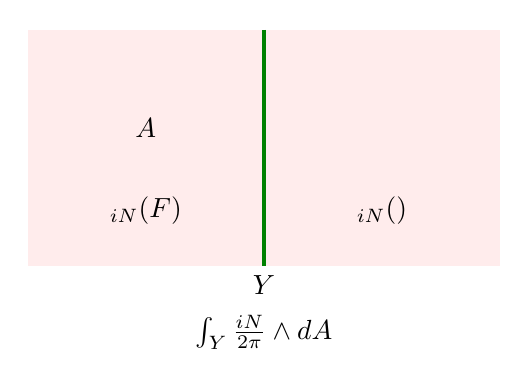
\begin{tikzpicture}
    \fill[pink!30!white] (-3, 2) rectangle (3, -1);
    \draw[green!50!black, ultra thick] (0,2)--(0,-1);
    \node at (0,-1)[below]{$Y$};
    \node at (0,-1.5)[below]{$\int_Y\frac{iN}{2\pi}\At \wedge dA$ };
    \node at (-1.5,1)[below]{$A$};
    \node at (-1.5,0)[below]{$\Lcal_{iN}(F)$};
    \node at (1.5,1)[below]{$\At$};
    \node at (1.5,0)[below]{$\Lcal_{iN}(\Ft)$};
  \end{tikzpicture}
  \caption{半空間ゲージ化により得られる欠陥の様子。}
  \label{fig:dualitydefectMaxwell}
\end{figure}
最後に$N=1$の場合についてコメントします。この場合は普通の対称性になります。この場合、Lagrangian密度として$\tau=i$で全体で\eqref{MaxwellDualTemp2}のものをとって考えるのが分かりやすいと思います。このとき全体で$\At,B$を積分すると全体で$\tau=i$のMaxwell理論が得られます。一方で、$D$の中では$A,B$を積分、$D$の外では$\At$を積分すると、$D$の外でも中でも$\tau=i$のMaxwell理論が得られますが、$Y=\del D$上で欠陥が現れます。この場合、積分のしかたが異なるだけなので、$D$の中に他の演算子が入っていないかぎり欠陥の期待値は$1$になります。したがってこの欠陥で表される一般化対称性は普通の対称性になります。

2次元の自由スカラー場でも似たような議論ができて、もっとよく調べられています。自己双対の点では半空間ゲージ化により得られる一般化対称性はやはり普通の対称性になります。この場合、実は対称性がもっと大きく拡大していて$\SU(2)\times \SU(2)$になっていることが知られています。4次元でこのような、さらに大きな拡大が分かると面白いと思います。
\end{document}